The XML benchmarking project XMARK~\cite{xmark/original} dataset is single record with large and complex tree structure. It is one of the most popular and most commonly used XML Benchmark~\cite{xmark/mlynkova2008xml}. It uses a small executable tool called  \textit{xmlgen} that enables to create a synthetic XML Dataset according to fixed DTD of an Internet auction database. The xmlgen produces the dataset that is platform independent and accurately scalable ranging from a minimal document to any arbitrary size limited by the capacity of the system. 

\subsubsection{Dataset}
\label{xmark-dataset}
	XMARK dataset is single record with huge and complicated tree structure ~\cite{xml/VIST}. 

\begin{figure}
	\centering
	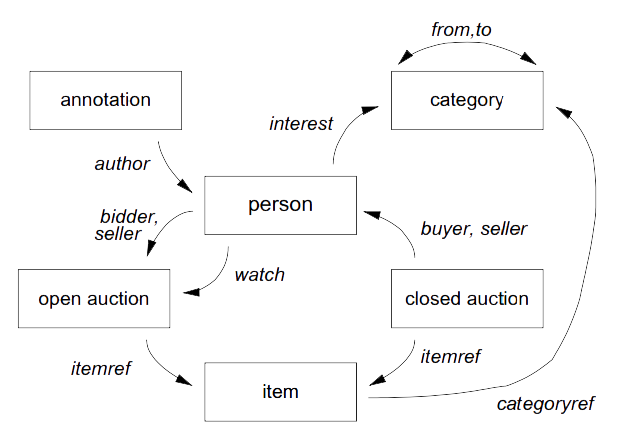
\includegraphics[width=0.47\textwidth]{img/xmark-references.png}{
		\label{xmark-reference}
	}
	\caption{Reference in \textit{XMark} dataset Fig~\cite{xmark/original}}
	\label{figParseProcess}
\end{figure}

\subsubsection{Queries}
\label{xmark-queries}
